\documentclass[11pt,a4paper]{article}
\usepackage{url} % \url command
\usepackage[export]{adjustbox} % Allow specifying image max dimensions
\usepackage{tabularx} % Tables which don't go off the edge of the page
\usepackage[british]{babel} % Quote characters
\usepackage[framemethod=tikz]{mdframed} % Boxes round text
\usepackage[space]{grffile} % Spaces in image filenames
\usepackage{breakurl}

% This turns off hyphenation
\tolerance=1
\emergencystretch=\maxdimen
\hyphenpenalty=10000
\hbadness=10000

% This allows URLs to span multiple lines
\renewcommand{\UrlBreaks}{\do\/\do\a\do\b\do\c\do\d\do\e\do\f\do\g\do\h\do\i\do\j\do\k\do\l\do\m\do\n\do\o\do\p\do\q\do\r\do\s\do\t\do\u\do\v\do\w\do\x\do\y\do\z\do\A\do\B\do\C\do\D\do\E\do\F\do\G\do\H\do\I\do\J\do\K\do\L\do\M\do\N\do\O\do\P\do\Q\do\R\do\S\do\T\do\U\do\V\do\W\do\X\do\Y\do\Z}

\title{MetaboClust User Guide}
\author{Martin Rusilowicz}

\graphicspath{{Images/userguide/}}

\newcommand{\menu}[1]{ \flqq\textit{#1}\frqq}
\newcommand{\icon}[1]{\includegraphics[height=0.75\baselineskip]{#1}}

\newenvironment{detailbox}[1][] {%
	\vspace{\baselineskip}
	\mdfsetup{
		frametitle={%
			\tikz[baseline=(current bounding box.east),outer sep=0pt]%
			\node[anchor=east,rectangle,fill=black!20]%
			{\strut #1};%
			\vspace{\baselineskip}%
		},
		%frametitlebelowskip=2cm,
		%innertopmargin=0pt,
		linecolor=black!50,
		topline=true,
		frametitleaboveskip=0pt,
		rightline=false,
	}
	\begin{mdframed}[]\relax
}
{
	\end{mdframed}
	\vspace{\baselineskip}
}

\begin{document}
\maketitle
\newpage

\section{System requirements}
For large datasets, a 64-bit system with 8Gb RAM is recommended. MetaboClust is dependent on the .NET framework. If you are running a recent version of Windows it is more than likely that this is already installed on your computer. If not you will need to download the installer version (see below), or download and install the Microsoft .NET framework from \url{https://www.microsoft.com/net/download}.

\section{Downloading binaries}

If the .NET framework is installed, download the most recent MetaboClust zip file from \\
 \url{https://bitbucket.org/mjr129/metabolitelevels_release}.  After downloading and unzipping, launch \textit{MetaboliteLevels.exe} to start the application.\\
\\
If the .NET framework is not already installed, a full installation, which includes the .NET framework, desktop and start-menu shortcuts and an un-installer, can be downloaded
instead. In this case download the most recent MetaboClust(installer) zip file. After downloading and unzipping, run \textit{Setup.exe} and follow the on-screen instructions. The application will be installed using Microsoft ClickOnce - for troubleshooting and details see \url{https://msdn.microsoft.com/en-us/library/t71a733d.aspx}. After the install you should be able to run the application from your start menu, or by launching \textit{MetaboliteLevels.exe} from the folder you installed the application to.

\begin{detailbox}[Note]
	If an error message appears when you try to start the application, check that the latest version of the .NET framework is installed and working.
\end{detailbox}

\section{Compiling from source}
If a full installation is preferred, which (if required) includes the .NET framework, desktop and start-menu shortcuts and an un-installer, the \textit{Installer} version can be downloaded instead.
MetaboClust is written in C\# using Visual Studio 2015. The source consists of three projects, all of which must be downloaded:\\
\\
\begin{tabularx}{\linewidth}{l X X X}
	\textbf{Project} & \textbf{Relative path} & \textbf{Contents} & \textbf{Download URL} \\ \hline
	MetaboliteLevels & \url{./MetaboliteLevels/MetaboliteLevels/MetaboliteLevels.csproj} & The main application & \url{https://bitbucket.org/mjr129/metabolitelevels} \\
	MChart & \url{./MChart/MChart/MChart.csproj} & Charting library & \url{https://bitbucket.org/mjr129/mchart} \\
	MGui & \url{./MGui/MGui/MGui.csproj} & Helper library & \url{https://bitbucket.org/mjr129/mgui} \\
\end{tabularx}
\\
\\
From the \textit{downloads} page of each of the projects, select \textit{download repository}. Unzip each of the downloads to a new folder on your disk. If any of the above libraries show as missing make sure they are present in the correct folder, or modify your solution to target the correct path.
\\
\\
MetaboClust also requires the following libraries. Initially these will show as \textit{missing}, but should be downloaded automatically by \textit{NuGet} during the first build. If you have disabled \textit{NuGet} in VS2015 you will need to add the libraries to the solution manually.

\subsection{Running the source}
Build and run the \textit{MetaboliteLevels} project to start the application. Note that due to optimisations being skipped, the application will run considerably slower if the build mode is set to \menu{debug} \textit{and/or} a debugger is attached.

\begin{itemize}
	\item MathNet.Numerics
	\item RDotNet
	\item JetBrains.Annotations
\end{itemize}

\section{Initial setup}
\label{section:ug_initial_setup}
\begin{center}
\includegraphics[max width=0.7\linewidth]{"Images/userguide/initial setup"}
\end{center}
When MetaboClust starts for the first time the initial setup screen shown above is presented and requires the following information to be entered:

\begin{detailbox}[Initial setup options]
	\begin{itemize}
	\item \textbf{Working directory} -- This is where the application stores its data. By default this is the application's home directory. The default value should suffice in most case but can be changed (e.g. if administrator permissions deny read-write access to that folder).
	
	\item \textbf{Path to R} -- MetaboClust uses \textsc{R} to operate and needs to know where R is located. Clicking the \menu{select} button to the right of the text box should automatically detect the location of R and present a drop-down list of the versions of R available. If MetaboClust cannot find an R installation, the path to R will need to be specified manually. Pressing the \menu{select} button (and then, if required, the \menu{browse} option) will prompt you to locate the R installation. On Windows, R is usually located at \texttt{C:\textbackslash Program Files\textbackslash R\textbackslash R-x.x.x\textbackslash bin\textbackslash x64}, where \texttt{x.x.x} is the version. This folder can be identified by the presence of the R library, \texttt{R.dll}.
	
	\item \textbf{Pathway tools databases} -- MetaboClust can use Pathway Tools databases to make identifications. If any databases are already present on the system MetaboClust can be directed to them here. If no databases are available the \menu{select} button will offer a default location which can be used to put the databases in when they are available.
	\end{itemize}
\end{detailbox}
When you are done, click the \menu{OK} button to commit the selections. MetaboClust detects the presence of errors on most screens. The software will check a connection to R can be established, and check to make sure it has read/write access to the data folders. A greyed out \menu{OK} button indicates an error and a small red arrow should point in the direction of anything amiss. Hover the mouse over the arrow for more details.

\section{Loading data}
\begin{center}
	\includegraphics[max width=0.7\linewidth]{"Images/userguide/loading data"}
\end{center}
Once the initial setup is completed the data-load screen shown above will appear. The 
\includegraphics[height=0.5\baselineskip]{Images/userguide/cog} icon in the bottom right of the window presents a drop down menu and the\menu{edit paths and libraries} option here will return you to the \textit{initial setup} screen.

\section{Creating a new session}
A MetaboClust ``session'' is a database comprising your data, annotations and analyses. You need to create a session before any analysis is performed. Select \menu{create a new session} on the data-load screen to create a new session. The application will walk you through its creation.

\begin{detailbox}[Important note]
	Clicking the \menu{show help} button (or in later versions the \icon{show help bar} icon) will show a \textit{\textbf{context sensitive}} help bar at the side of the screen containing up-to-date details of the input fields.  For inputs requesting files the \menu{show file format details} button within the help bar describes the expected layout of input files.
\end{detailbox}
Clicking the \menu{Next} button progresses to the next stage of input. If this greyed out a small red arrow will point to anything amiss. Hovering the mouse over the arrow should describe the problem.

\begin{detailbox}[Loading data]
	\begin{itemize}
		\item \textbf{Template} -- Allows you to start from a previous setup. Normally you will start with the \menu{blank template}.
		\item \textbf{Session name} -- For your reference only
		\item \textbf{Data set}
		\subitem \textbf{Data source} -- If you have LC-MS data MetaboClust needs to know how the adducts are formed. If the data is not sourced from LC-MS, or automated annotations are not required, then select \menu{Source = Other}, otherwise select the column mode (positive or negative). The \menu{Source = Mixed mode} option allows you to mix modes, but your\menu{peaks} file must then contain an extra column specifying the mode of each peak (\menu{1} or \menu{-1}).
		\subitem \textbf{Data matrix} -- The data matrix is a grid containing the recorded intensities, with 1 row per observation and 1 column per variable (peak). Row and column names must be provided and must specify unique names for all observations (which can be O1, O2, O3,... for example) and variables (V1, V2, V3, ... for example). See the help bar as described above for exact details.
		\subitem \textbf{Observation information} -- The observation information matrix gives details for each observation, with one observation on each row and one field of information in each column. Row namess should contain the observation IDs as specified for the \menu{Data} matrix and column headers should contain the field names. Most fields are optional, but some features do require specific fields (for instance batch correction requires the \menu{batch} and/or \menu{acquisition order} fields). Since the exact file format may change with a new release, please see the help bar in the software itself for the list of fields (column headers) available.
		\subitem \textbf{Peak/variable information} -- The peak/variable information matrix gives details for each covariate. The software refers to these variable as peaks to avoid ambiguity with other variables, such as algorithm parameters. Please see the help bar for the list of fields available.
		\subitem \textbf{Alternate intensities} -- Sometimes another version of your data may be available, e.g. scaled or unscaled, normalised or raw. The alternate intensities option allows this to be loaded in for quick reference later. This data can be viewed, but it will not be used in the actual analysis. This feature is not present from version 1.2 onwards as an unlimited number of intensity matrices can be loaded from the file menu.
		\subitem \textbf{Condition names} -- If your experimental groups do not have intuitive names, e.g. just ``1'', ``2'' and ``3'', then this allows them to be mapped to more informative names.
		\item \textbf{Conditions}
		\subitem \textbf{Specify conditions} -- Details of the experimental groups can be provided here. The conditions should be the same as in the \textit{observation information} file or, if present, the \textit{condition names} file. This information is not mandatory, but if specified  will allow the software to generate default statistics and filters (described later). Conditions can also be added manually later.
		\item \textbf{Statistics}
		\subitem \textbf{Auto-create statistics} -- If  conditions have been specified, $t$-tests between experimental groups and controls, as well as Pearson correlations of the intensities for each group against time, can be generated. These options are not available if conditions were not specified, but can be calculated later.		
		\subitem \textbf{Perform corrections} -- The UV-scale and centre data correction can be added to your pipeline here. This and other corrections can also be added or modified later.
		\item \textbf{Compound libraries} -- These are the compound and pathway libraries used for annotations and pathway analysis. One or more of these must be selected to enable automated annotations. If you don't have any libraries on your system then the list will be empty.
		\subitem \textbf{Adduct libraries} -- Adduct libraries are used for automated annotations. There are two adduct libraries built into MetaboClust, \textit{All} and \textit{Refined}. All adducts listed on http://fiehnlab.ucdavis.edu/staff/kind/Metabolomics/MS-Adduct-Calculator (Kind, 2016) are incorporated in the \textit{All} library with a subset in the \textit{Refined} library.
		\item \textbf{Automated identification} -- Peaks can be annotated with potential metabolite identifications. For this option to be selected the \menu{tolerance}  and \menu{annotation status} must be specified. Possible annotation statuses are \menu{tentative} \\
		(unconfirmed), \menu{affirmed} (computationally confirmed) or \menu{confirmed} (experimentally confirmed).
		\subitem \textbf{Peak-peak matching} -- This annotates peaks with other peak IDs based on $m/z$ similarity and is primarily used to search for related compounds.
		\subitem \textbf{Manual identifications} -- Manual identifications can be uploaded. See the help bar for the exact file format. The \menu{annotation status} specified here will only be used if that information is missing from the file itself.
	\end{itemize}
\end{detailbox}
When all the fields you wish to select are complete click the \menu{OK} button to load the data. This may take a few minutes, especially if automated peak-compound annotations are being performed. Saving the session will avoid this delay in future.

\section{Data exploration}
\begin{center}
	\includegraphics[max width=0.7\linewidth]{"Images/userguide/main screen"}
\end{center}
Once you have created or loaded a session you will be presented with the main screen, shown above. There is no fixed series of steps in data analysis, but a brief overview of possibilities will be presented here. The images shown are taken from the analysis of the \textit{Medicago} leaf data, provided as a sample data set. This LC-MS dataset (negative mode) is provided as a sample data set and comprises 184 observations and 2920 peaks, with four experimental groups, C (Control), D (Droughted), F (Fusarium treated), and B (Both Fusarium treated and Droughted), as well as QC samples. Peaks were automatically annotated using the MedicCyc database (Urbanczyk-Wochniak et al., 2007, Bioinformatics 23(11), pp 1418-1423).

\section{Univariate statistics}
\label{section:ug_univariate}
Double clicking a peak in the list to the top-left of the window will present a plot of the chosen peak should be displayed to the right. This is a useful first step to ensure the data has loaded correctly.

\begin{detailbox}[Graph controls]
	\begin{itemize}
		\item \textbf{Left or right click} -- Select point or series. Details on that point will be displayed above the graph. Repeatedly clicking will cycle through the display options.
		\item \textbf{Left click and drag} -- Box-zoom
		\item \textbf{Mouse wheel} -- Zoom in or out
		\item \textbf{Middle click }-- Restore zoom and cancel selection.
	\end{itemize}	
	
	The \menu{plot} button above the graph provides plotting options, including exporting the plot to a file and toggling display of the legend.
\end{detailbox}
To show more information about each peak, click the \icon{columns} icon above the peak list. In the example below, a particular statistic is chosen for display. The p-value for the t-test between experimental group G and the control group is denoted p.G and the Pearson correlation between the intensities for group G with time is denoted r.G.

\begin{center}
	\includegraphics[max width=0.5\linewidth]{"Images/userguide/column edit"}
\end{center}
The values  of the chosen statistic for each peak will be displayed in a new column and the peaks can then be sorted on these values by clicking on the column header to allow  the most ``significant'' peaks to be located.

\begin{center}
	\includegraphics[max width=0.5\linewidth]{"Images/userguide/column header"}
\end{center}
Clicking \menu{view as heatmap} will display the column as a heatmap with brighter colours indicated higher values. Note that heat-map is ordered the same as the column, so if the peaks have been sorted by this column , the heat-map will appear as a gradient.

\begin{center}
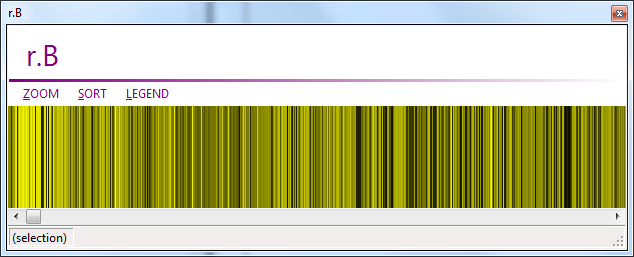
\includegraphics[max width=0.7\linewidth]{Images/userguide/heatmap}
\end{center}
To add univariate statistics at this point, click the \icon{stats} \menu{stats} option from the tool-bar, or select \menu{Database/Workflow/Statistics} from the menu.

\begin{center}
\includegraphics[max width=0.7\linewidth]{"Images/userguide/statistics list"}
\end{center}
Select \menu{New} to create a new statistic and the window below will appear.

\begin{center}
	\includegraphics[max width=0.7\linewidth]{"Images/userguide/new statistic"}
\end{center}

\begin{detailbox}[Statistic fields]
	\begin{itemize}
		\item \textbf{Title} -- A title for the statistic. A name will be provided for you if you don't specify one. Clicking the \icon{comment} icon provides space to add detailed comments.
		\item \textbf{Method} -- The statistic to calculate, click the \icon{database} button to the right of the method to define your own methods.
		\item \textbf{Parameters} -- If the method takes any parameters, enter them here. Multiple parameters are separated by commas. Clicking the button next to the text-box displays the parameters as individual inputs rather than a single-line text-box.
		\item \textbf{Target} -- The intensity matrix for which the statistics are to be calculated. This may be from various stages of the analysis: ``origin'' indicates the original intensity matrix that was loaded and will be the only option until data-correction has been performed. Items marked with an asterisk designate dynamic sources. Pre-version 1.2 only two intensity matrices are available, being the latest set of observations (\menu{*final correction}) and latest trend (\menu{*final trend}).
		\item \textbf{For} or \textbf{Compare} -- Selects the filter to define the set of observations to be used in the test/comparison. Click the \icon{database} button to define new filters.
		\item \textbf{Against} -- Only available for bivariate statistics, specifies the second input vector:
		\subitem \textbf{The corresponding time} -- The times corresponding to the first input vector (e.g. to correlate intensity against time)
		\subitem \textbf{A different peak} -- The set of intensities corresponding to the first input vector for a different peak (e.g. to find similar peaks)
		\subitem \textbf{The same peak} -- The set of intensities sourced from different observations on the same peak (e.g. to contrast experimental and control observations).
	\end{itemize}
\end{detailbox}
For example, to calculate the mean of the QC samples select \menu{Method = Mean} and \menu{For = Group is Q}. The \menu{Preview} box allows you to preview the result of your calculation on individual peaks. Select \menu{OK}.
Click \menu{OK} again to leave the \menu{List editor}. Any new or modified statistics will be recalculated. Edit the columns for the peaks list to show your new statistic.

\section{Using additional R packages and user-defined scripts}

Users own scripts for statistics, metrics or trends can be added via the new statistics window. To do this, click the \icon{database} next to the method box, and then, rather than choosing from the list of available options, click \menu{new} which will open the script editor as in the example below. 

\begin{center}
	\includegraphics[max width=0.7\linewidth]{"Images/userguide/newscript"}
\end{center}

The script for any available R package could be added this way. 

\section{Exploring annotations}
\begin{center}
	\includegraphics{"Images/userguide/database contents"} 
\end{center}
The set of coloured icons above the list allows paging between the database contents. If automated annotation was chosen when loading the data try selecting the \icon{annot}
 tab and viewing the annotations.
 Double click an annotation to view it. As there are no graphs associated with annotations, nothing will be displayed in the top-right, but the secondary list in the bottom-left should update to reflect the selected annotation. Above the secondary list select the \menu{peak} tab to display the peaks associated with the selected annotation. Double-click the peak which appears in the list to plot the peak associated with the annotation.

\begin{detailbox}[Data exploration]
Almost all of the data in MetaboClust can be explored in this way. The primary list (top) selects items within the dataset, whilst the secondary list (bottom) allows you to explore items within the context of the primary selection. To select an item in the secondary list as the primary selection, click its title above the list:
	\begin{centering}
	\includegraphics[max width=0.7\textwidth]{"Images/userguide/promote selection"}
	\end{centering}
	
\end{detailbox}	

\section{Multivariate statistics}
An overview of your data can be obtained using PCA. Click the \icon{pca} button in the menu strip to launch the PCA window.

\section{MVA}
The MVA window presents a PCA plot of the dataset. The options to the left control the method of PCA and the display of the scores.

\begin{detailbox}[MVA controls]
	\begin{itemize}
		\item \textbf{Method} -- Switch between PCA and PLSR plots
		\item \textbf{Source} -- Perform the analysis on observations or variables (peaks)
		\item \textbf{View} -- Toggle between scores and loadings plots.
		\item \textbf{Legend} -- Select what the colours on the graph represent.
		\item \textbf{Corrections} -- View your data with various corrections.\footnote{\label{note:abct} Corrections and trends are defined from the main screen.}
		\item \textbf{Input} -- Choose between performing PCA of all observations, or just your trend line (useful for noisy datasets).
		\item \textbf{Observations} -- Select a filter to determine the set of observations to explore.
		\item \textbf{Peaks} -- Select a filter to determine the set of peaks to explore.
		\item \textbf{View on main} -- Displays the selected peak or observation on the main screen.\footnote{\label{note:aspo} Requires an object in the plot to have been selected first}
		\item \textbf{Mark as outlier} -- Applies a filter to exclude the selected observation. 
		\item \textbf{Next component} -- Views the next principal component. 
		\item \textbf{Previous component} -- Views the previous principal components
		\item \textbf{Plot options} -- Displays the set of plot options, including toggling display of the legend.
	\end{itemize}
\end{detailbox}
For example, if the data were collected in batches, click the \textsc{Legend} -- the \textsc{Batch} to colour the plot by batch.
Subsets of the data can be selected using filters.  Click the \textsc{Observations} menu to show a list of observation filters by experimental group. As when creating a new statistic, if no filters are available you can click \menu{Observations/Edit observation filters...} to create a new filter. The same can be done with peak filters by selecting \menu{Peaks/Edit peak filters...}.\\
PCA can also be used for outlier removal. Click an observation in the plot and select the \textsc{mark as outlier} button. A new filter will be created, excluding that observation (or peak) from the dataset.

\section{Data correction}
\label{section:ug_data_correction}
Select \menu{Correct} from the menu-bar of the main screen to open the corrections list. Click \menu{new} to create a new one. \\
The data correction window presents a list of data-correction methods, as well as trend generation methods. Data-correction methods, such as "UV scale and centre" act alone, whilst the trend-generators can be used to perform batch correction and control correction.

\begin{detailbox}[Data correction options]
	\begin{itemize}
		\item \textbf{Title} -- A title for the correction method. A name will be provided for you if you don't specify one. Clicking the \icon{comment} icon provides space to add detailed comments.
		\item \textbf{Source} -- Data on which to perform the correction.
		\item \textbf{Method} -- The correction to be performed. Click the \icon{database} button to the right of the method to define your own methods.
		\item \textbf{Parameters} -- If the method takes any parameters, enter them here. Multiple parameters are separated by commas. Clicking the button next to the text-box displays the parameters as individual inputs rather than a single-line text-box.
		\item \textbf{Operator} -- \textit{Only available for trend-based corrections.} The correction takes the form $x\prime = f(x, t)$, where $f$ is defined as divide or subtract. Generally a batch correction will use \menu{divide} and control correction \menu{subtract}.
		\item \textbf{Filter} -- \textit{Only available for trend-based corrections.} Selects the set of points used to generate the trend.
	\end{itemize}
\end{detailbox}
The preview window allows you to preview the correction on an individual peak. For trend-based corrections the trend used will be highlighted to the left.

\subsection{Examples}

\subsubsection{QC correction}
Dividing by the mean of the QC samples in the batch is a fairly standard method of correcting for batch-differences in LC-MS, to use this select: \menu{Method = straight line across mean}, \menu{Corrector = Batch}, \menu{Operator = Division} and \menu{Filter = Group is Q}. 

\subsubsection{Background correction}
To perform background correction, as described in Rusilowicz et al., (2016) Metabolomics 12(3), pp 1-11, select \menu{Method = moving median}, \menu{Corrector = Batch} and \menu{Filter = All}. You will need to enter the window width \menu{w} parameter in this case. Experiment with values to find one that looks good in the plot.

\subsubsection{Scale and centre}
Select \menu{Method = UV scale and centre}. This correction should generally be performed \textit{after} batch correction and therefore the \menu{Source} parameter should point to the intensity matrix generated by your batch correction -- QC or Background correction as described above.

\subsection{Viewing corrections}
\begin{center}
	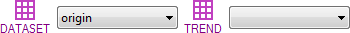
\includegraphics[max width=0.7\linewidth]{Images/userguide/dataset}
\end{center}
Back on the main screen you will need to select your corrected dataset before your changes can be viewed. Click \icon{dataset button} \menu{dataset} or the drop-down list next to it to select your modified data. You can use the \menu{*Final correction} meta-option to always keep your display up-to-date with the latest correction.

\section{Trend line generation}
A trend can be generated across observations to be used for background correction or clustering observations, or a trend can be obtained for each variable by averaging over the replicates. Select \icon{trend} \menu{trend} from the tool-bar or \menu{Database/workflow/trends} to define a trend.
You will be presented with a list much like the \menu{correction} window. (Pre-version 1.2 this will contain a \menu{no-trend} entry, click \menu{remove} to get rid of it). Click \menu{new} to create a new trend.

\begin{detailbox}[Trend options]
The \menu{New trend} options are largely the same as those described in section \ref{section:ug_data_correction}.
\end{detailbox}

\subsection{Example}

The simplest trend is the mean for each time-point. Select \textsc{Method = moving mean} with value \textsc{w = 1}. (\textsc{w} is the window width for the moving mean --  a window width of 1 effectively the mean of the replicates).

\subsection{Viewing trends}
Back on the main screen you will need to select your trend before your changes can be viewed. Click\menu{trend}
 or the drop-down list next to it to select your modified data. You can use the \menu{*Final trend} meta-option to keep your display up-to-date with the latest correction.
After selecting your trend any peaks you plot will show the specified trend. You may see bold lines through 0 on peak plots pre-version 1.2 before a trend line has been defined. 

\section{Clustering}
Clusters are created in the same way as corrections, statistics or trends. Select the \menu{Cluster} option from the tool-bar of the main window.

\begin{detailbox}[Clustering options]
	\begin{itemize}
		\item \textbf{Title} -- A title for the cluster analysis. A name will be provided for you if you don't specify one. Clicking the \icon{comment} icon provides space to add detailed comments.
		\item \textbf{Method} -- The clustering algorithm to be performed. Click the \icon{database} button to the right of the method to define your own methods.
		\item \textbf{Parameters} -- If the method takes any parameters, enter them here. Multiple parameters are separated by commas. 
		\item \textbf{Peaks} -- Which peaks to cluster. A filter can be defined by selecting the \icon{database} icon next to the list.
		\item \textbf{Distance} -- The distance metric to be used to calculate statistics on clustering performance(next option).
		\item \textbf{Parameters} -- Parameters required for the distance metric.
		\item \textbf{Statistics} -- Statistics to calculate on clustering performance.
		\item \textbf{Source} -- Data on which to perform the correction.
		\item \textbf{Observations} -- The set of observations to use in the clustering vectors.
		\item \textbf{One vector per experimental group} -- Normally one vector is created per-peak, select this option to ``split'' the peaks into one vector for each experimental group.
		\item \textbf{Parameter optimiser} -- If the clustering algorithm takes parameters this option can be used to optimise them using statistics such as \textit{silhouette width} or \textit{BIC}.
	\end{itemize}
\end{detailbox}

\subsection{Viewing clusters}
On the main screen click the \menu{cluster} icon above the primary list to view the clusters. Double click a cluster to plot it in the cluster plot area. Note that clusters are always plotted using the vectors with which they were created, so the \menu{trend} and \menu{dataset} visual options will have no effect on the cluster plot.\\
Clicking a vector within the cluster plot will select the peak associated with that vector as the secondary selection. Alternatively, select the \menu{peaks} tab from the secondary list to show a list of peaks assigned to the selected cluster. Double clicking a peak in this list will plot the peak and highlight it in the cluster plot.

\begin{center}
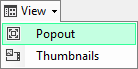
\includegraphics{Images/userguide/popout}
\end{center}
If you want to see a quick overview of all clusters, then click the \menu{View} and \menu{Popout} options above the list of clusters. By default each plot is scaled to fit the plot area, so flat clusters may appear as noisy. To change this and scale all clusters to the same Y-axis, change the plot options by going to the \menu{Prefs} window and setting the \menu{Cluster} -- \menu{Y-axis range} to \menu{Scale to matrix}.

\subsection{Metabolite and pathway exploration}
With a cluster selected, clicking the \menu{compounds} or \menu{pathways} options will show compounds and pathways potentially highlighted by that cluster. Double-clicking these compounds or pathways will highlight the overlap between them and the cluster in the cluster plot. You can show or hide the degree of overlap, or sort clusters by overlap, by selecting the \icon{columns} icon in the secondary list.\\
A reverse exploration can also be performed, selecting a \menu{pathway} or \menu{compound} in the primary list will plot the trends of the peaks associated with the pathway or compound in the cluster plot. (You can change the \menu{dataset} or \menu{trend} in this case.) As for the clusters, selecting individual trends will plot the actual peak. Selecting \menu{clusters} in the secondary list will show the clusters affected by peaks annotated with the pathway or compound.

\section{General options}

\begin{itemize}
	\item Show or hide observations from experimental groups -- Click the group icon in the main tool-bar to toggle group visibility, or select the \icon{groups} \menu{groups} icon.
	\item Rename groups, peaks, etc. -- Select the \menu{Database} menu to show the database, then edit the group or peak. The groups database can be accessed quickly from the \icon{groups} \menu{groups} icon in the tool-bar. Clicking the name of the session in the top-right of the main screen allows you to rename the session.
	\item Change display options -- Select the \icon{prefs} icon from the tool-bar.
	\item Find out which files were used to create a session -- Select \menu{Help/Session information} from the main menu
	\item Find an individual item -- Click the \menu{name} column of the peaks list and select \menu{filter} from the menu to search for individual items.
	\item Get an overview of the session, including peak and observation counds -- Select \menu{View/Miscellaneous functions} and then \menu{View statistics} from the window that appears.
\end{itemize}

\section{Known bugs}
MetaboClust is beta software. A list of known bugs is maintained on the download page. Please submit any bugs you find to this list.

\end{document}